\documentclass[education,article,submit,moreauthors]{Definitions/mdpi}

\firstpage{1}
\makeatletter
\setcounter{page}{\@firstpage}
\makeatother
\pubvolume{1}
\issuenum{1}
\articlenumber{0}
\pubyear{2026}
\copyrightyear{2026}
\datereceived{}
\daterevised{}
\dateaccepted{}
\datepublished{}

\usepackage{fontspec}
\usepackage{polyglossia}
\setmainlanguage{english}
\setotherlanguage{arabic}
\newfontfamily\arabicfont[Script=Arabic,Scale=1.1]{Geeza Pro}
\setlength{\headheight}{20pt}

\Title{Efficient Arabic Text Simplification for Moroccan IT Education via Glossary-Guided LoRA Fine-Tuning}
\title{Efficient Arabic Text Simplification for Moroccan IT Education via Glossary-Guided LoRA Fine-Tuning}
\Author{Khalid Essaadani $^{1,*}$ and Soumia Ziti $^{1}$}
\author{Khalid Essaadani and Soumia Ziti}
\AuthorNames{Khalid Essaadani and Soumia Ziti}
\address{%
$^{1}$ \quad Mohamed V University in Rabat, Rabat, Morocco; khalid\_essaadani@hotmail.fr}
\corres{Correspondence: khalid\_essaadani@hotmail.fr}

\abstract{In Morocco, many learners encounter information technology (IT) content through French or English, while their strongest language of conceptual understanding is often Arabic. This linguistic gap increases cognitive load and reduces comprehension. This paper presents a lightweight approach for simplifying IT educational content into clear Modern Standard Arabic using a fine-tuned small language model. The system is based on Qwen2.5-1.5B-Instruct and fine-tuned using LoRA on a custom dataset of 150 paired examples covering major IT domains. A domain glossary was integrated into prompt construction to improve terminology consistency. Evaluation on 20 unseen prompts shows consistent improvements: fluency (3.15 $\rightarrow$ 4.25), meaning preservation (3.35 $\rightarrow$ 4.35), simplicity (3.05 $\rightarrow$ 4.20), and terminology accuracy (3.15 $\rightarrow$ 4.15). The results demonstrate that glossary-guided fine-tuning is an effective strategy for improving native-language accessibility of IT education in multilingual contexts such as Morocco.}

\keyword{Arabic NLP; text simplification; IT education; Morocco; glossary-guided prompting; LoRA fine-tuning; multilingual education}

\begin{document}
\section{Introduction}

Language is a central factor in educational access, especially when learners are expected to study technical content through a language that is not the one in which they most naturally construct meaning. In multilingual educational settings, the language of instruction can add an additional burden that is separate from the conceptual difficulty of the subject itself. Research on multilingual and mother-tongue-based education has consistently shown that learning in a familiar language improves comprehension, participation, and inclusion, while unfamiliar instructional languages may reduce learners’ ability to engage fully with academic content \citep{Ichou2022PromotingQuality,Ouchaib2021LanguageInstructionScience,Hassen2021LearningDifficultiesMedicine}.

This issue is particularly important in Morocco, where scientific and technical education has long been shaped by a multilingual but unequal linguistic configuration involving Arabic, French, and increasingly English \citep{Ichou2022PromotingQuality,Jarmouni2024ImpactInstructionLanguage,Mohammed2024LanguagePolicyDisturbances}. In practice, many learners encounter technical and scientific explanations through French or English, while their strongest language of conceptual access is often Arabic \citep{Ouchaib2021LanguageInstructionScience,Hassen2021LearningDifficultiesMedicine}. As a result, students may have to process two layers of difficulty at once: the technical concept itself and the linguistic code used to explain it. In information technology (IT) education, this challenge becomes especially visible because many expressions such as \textit{inheritance}, \textit{query}, \textit{firewall}, and \textit{cloud computing} are not merely isolated vocabulary items, but concept-bearing units whose misunderstanding can directly affect learning.

One possible way to reduce this barrier is text simplification. Unlike literal translation, simplification seeks to preserve the original meaning while rewriting content in a clearer, shorter, and more pedagogically accessible form. In educational settings, simplification may involve reducing lexical difficulty, restructuring sentences, clarifying discourse organization, and stabilizing technical terminology. Recent work describes text simplification as operating across lexical, syntactic, and broader discourse-oriented levels, while contemporary systems increasingly rely on neural and Transformer-based models to perform controlled rewriting \citep{Bahrainian2024AdaptiveTeaching,AlThanyyan2021AutomatedTextSimplification}.

At the same time, recent advances in artificial intelligence, natural language processing, and large language models have opened new possibilities for adaptive learning, personalized educational support, and more accessible forms of content delivery \citep{Alqahtani2023EmergentRoleAI,Gutierrez2023AILanguageEducation,RE2024RevolutionizingEducationAI,Ismaili2024AILiteracyAdaptiveLearning}. In the Arabic NLP space, emerging work on Moroccan and regional Arabic varieties further suggests that low-resource language adaptation is becoming increasingly feasible. Models such as Atlas-Chat and GemMaroc show that dialect-aware adaptation for Moroccan Arabic can be achieved with increasingly practical methods, while recent resource-aware work also demonstrates that Arabic-focused model adaptation can be performed efficiently on modest hardware \citep{Shang2024AtlasChat,Skiredj2025GemMaroc,Aryan2024ResourceAwareArabicLLM}. However, these advances do not directly solve the problem of educational simplification of technical content for Moroccan learners. General-purpose models often produce unstable terminology, multilingual drift, or outputs that remain too literal or too complex for instructional use.

This reveals a concrete need for a lightweight, domain-aware, and educationally grounded simplification system that can rewrite IT explanations into clear Arabic while preserving technical meaning. Such a system is particularly relevant in contexts where large-scale computational infrastructure may be unavailable and where pedagogical usefulness depends not only on fluency, but also on conceptual fidelity and terminology consistency \citep{Aryan2024ResourceAwareArabicLLM,Kolchenko2018AIReplaceTeachers,Talib2023MTechnologiesCareerGuidance}.

To address this need, this paper proposes a glossary-guided fine-tuning approach for Arabic IT text simplification. The study develops a compact prototype built on Qwen2.5-1.5B-Instruct \citep{Qwen2024TechnicalReport,Qwen2024ModelCard} and adapts it through LoRA fine-tuning on a small curated dataset of technical explanations paired with simplified Arabic outputs. In addition, a domain glossary is integrated into prompt construction in order to improve terminology stability and reduce lexical inconsistency during generation. The aim is not literal translation, but pedagogical rewriting: preserving technical meaning while producing clearer Arabic explanations that are more accessible to Moroccan learners.

The contributions of this paper are fourfold. First, it introduces a compact Arabic IT simplification dataset built from paired original technical explanations and simplified Arabic targets across major IT domains. Second, it proposes a glossary-guided prompt-construction strategy to improve the consistency of Arabic technical terminology during model adaptation. Third, it demonstrates that a small instruction-tuned language model can be adapted effectively for a specialized Arabic educational task using parameter-efficient fine-tuning. Fourth, it provides empirical evidence that this approach improves fluency, meaning preservation, simplicity, and terminology accuracy in the simplification of technical educational content.

By treating multilingual difficulty in Moroccan technical education not only as a language-policy issue but also as an applied NLP and instructional design problem, this study offers a practical framework for improving native-language accessibility in IT learning. In doing so, it contributes to ongoing efforts to make technical education more comprehensible, equitable, and instructionally accessible in multilingual contexts.

\begin{figure}[H]
\centering
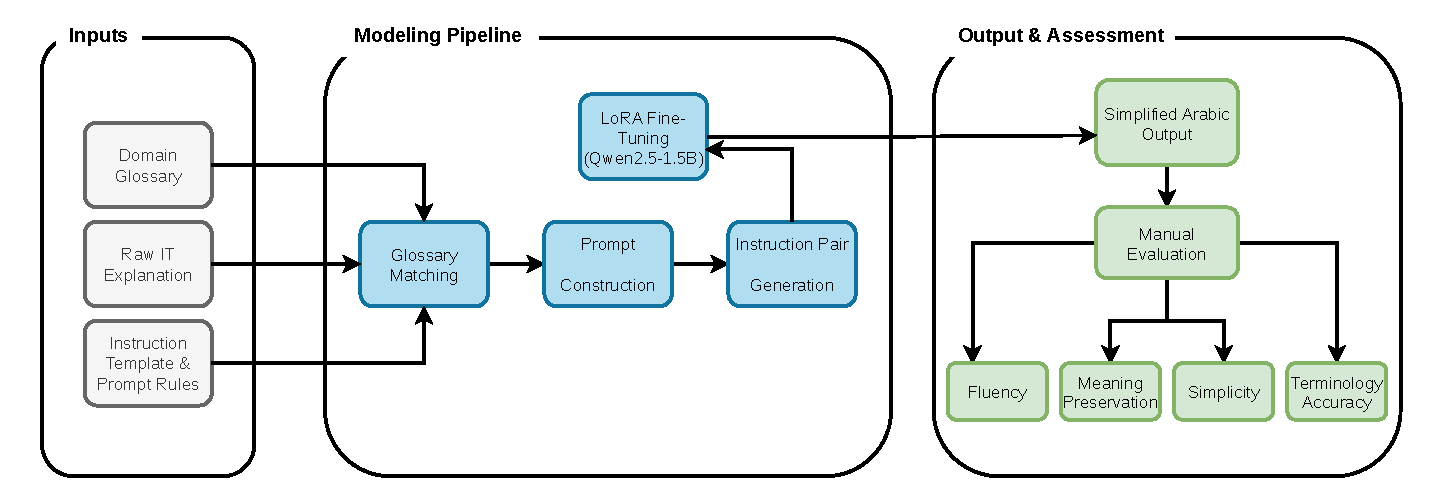
\includegraphics[width=\linewidth]{simplification-pipeline.pdf}
\caption{Glossary-guided Arabic IT simplification pipeline.}
\label{fig:arch}
\end{figure}

\section{Related Work}

Research relevant to this study falls into four intersecting areas: language of instruction in Moroccan education, AI in education, Arabic and Darija language modeling, and text simplification for educational accessibility.

Morocco’s linguistic environment is highly multilingual, involving Modern Standard Arabic (MSA), Moroccan Arabic (Darija), Amazigh, French, and increasingly English \citep{Fathi2024DualDiglossia,Loutfi2020MotherTongues,Boussagui2025LanguagePolicy,Farissi2025LanguageIssues}. In formal education, Arabic and French have historically occupied unequal but complementary roles, with French maintaining particular dominance in higher education and in scientific and technical disciplines \citep{Errihani2017EnglishEducation,Chihab2024AttitudesInstruction,Boussagui2025LanguagePolicy}. This configuration has repeatedly been associated with barriers to comprehension, performance, self-confidence, and educational continuity, especially when students move from Arabic-medium schooling into French-medium scientific study \citep{Ichou2022PromotingQuality,Jarmouni2024ImpactInstructionLanguage,Ouchaib2021LanguageInstructionScience,Mohammed2024LanguagePolicyDisturbances}. At the same time, classroom practice often relies informally on Darija to support explanation and understanding, suggesting that learners’ actual linguistic repertoires remain central to educational access \citep{Ichou2022PromotingQuality,Kroon2003MotherTongue,Loutfi2020MotherTongues}.

\section{Research Gap}

Despite growing interest in language policy, multilingual education, and artificial intelligence in Morocco, an important gap remains at the intersection of these domains. Existing studies have documented the linguistic barriers Moroccan learners face when studying scientific and technical content through non-native instructional languages \citep{Ichou2022PromotingQuality,Jarmouni2024ImpactInstructionLanguage,Ouchaib2021LanguageInstructionScience,Mohammed2024LanguagePolicyDisturbances}. Other work has explored the broader educational role of AI, including adaptive learning, AI literacy, and personalized support \citep{Alqahtani2023EmergentRoleAI,Gutierrez2023AILanguageEducation,RE2024RevolutionizingEducationAI,Ismaili2024AILiteracyAdaptiveLearning}. However, these strands remain only loosely connected, and there is still limited work on concrete NLP systems designed to simplify technical educational content into accessible Arabic for Moroccan learners.

More specifically, the literature lacks domain-specific simplification systems for Arabic technical education in Morocco. While recent work on Moroccan and regional Arabic varieties shows that dialect-aware language modeling and low-resource adaptation are becoming increasingly feasible \citep{Shang2024AtlasChat,Skiredj2025GemMaroc,Mahdi2025TunisianArabicLLMs,Aryan2024ResourceAwareArabicLLM}, these studies do not directly address pedagogical rewriting of technical material, nor do they provide lightweight educational pipelines that combine terminology control, parameter-efficient adaptation, and evaluation focused on pedagogical quality. Existing work rarely integrates glossary-guided data preparation, efficient fine-tuning, and learner-oriented evaluation dimensions such as fluency, meaning preservation, simplicity, and terminology accuracy.

This study addresses these gaps by proposing a lightweight Arabic text simplification approach for IT education in Morocco based on a small instruction-tuned language model, glossary-guided dataset construction, and LoRA fine-tuning. Rather than treating multilingual difficulty only as a language-policy issue, the present work operationalizes it as an applied NLP and instructional design problem, and contributes a practical framework for making technical educational content more comprehensible and instructionally accessible to Moroccan learners.

\section{Methods}

\subsection{Research Design}

This study followed a computational prototype design. It did not involve classroom experiments, interviews, surveys, or direct participation by students or teachers. Instead, the work focused on the construction of a simplification dataset, the fine-tuning of a small open language model, and the evaluation of generated outputs through a rubric-based comparison against the base model.

The core task was defined as follows:

\begin{itemize}[leftmargin=1.5em]
    \item \textbf{Input:} a French or technically dense IT explanation
    \item \textbf{Output:} a simplified Arabic explanation suitable for Moroccan learners
\end{itemize}

The objective was not literal translation. The target was pedagogical simplification: preserving technical meaning while making the explanation clearer, shorter, and easier to understand.

\subsection{Dataset Construction}

A custom dataset of 150 paired examples was created for this study. Each example contained an original technical explanation and a corresponding simplified Arabic version. The dataset spans ten IT domains, including programming fundamentals, object-oriented programming, algorithms, databases, web development, networking, operating systems, software engineering, cybersecurity, and cloud computing. The distribution of examples across domains and difficulty coverage is shown in Table~\ref{tab:dataset_distribution}.

Each data row included topic metadata, source language, keywords, and difficulty level. The dataset was organized in CSV format and then converted into JSONL for instruction tuning.

The target simplifications were written in Modern Standard Arabic according to three principles: (1) preserving the exact technical meaning, (2) simplifying wording and sentence structure, and (3) preferring clear Arabic technical terminology.

The dataset was intentionally small but curated, because early experiments showed that terminology consistency mattered more than simply increasing the number of examples.

\begin{table}[H]
\caption{Dataset distribution by IT domain and difficulty coverage.}
\label{tab:dataset_distribution}
\centering
\begin{tabular}{lcc}
\toprule
Domain & Number of Examples & Notes \\
\midrule
Programming Fundamentals & 5  & Easy only \\
Object-Oriented Programming & 5  & Easy, Medium \\
Algorithms & 20 & Easy, Medium, Hard \\
Databases & 20 & Easy, Medium \\
Web Development & 20 & Easy, Medium \\
Networking & 20 & Easy, Medium \\
Operating Systems & 10 & Easy, Medium \\
Software Engineering & 20 & Easy, Medium \\
Cybersecurity Basics & 10 & Easy, Medium \\
Cloud Computing Fundamentals & 20 & Easy, Medium \\
\bottomrule
\end{tabular}
\end{table}

\subsection{Glossary-Guided Prompt Construction}

A domain glossary was created to improve terminology stability during training. The glossary mapped French and, when available, English technical terms to preferred Arabic equivalents. Examples included:

\begin{itemize}[leftmargin=1.5em]
    \item \textit{classe} $\rightarrow$ \textarabic{صنف}
    \item \textit{objet} $\rightarrow$ \textarabic{كائن}
    \item \textit{héritage} $\rightarrow$ \textarabic{وراثة}
    \item \textit{requête} $\rightarrow$ \textarabic{استعلام}
    \item \textit{serveur} $\rightarrow$ \textarabic{خادم}
    \item \textit{pare-feu} $\rightarrow$ \textarabic{جدار ناري}
    \item \textit{CDN} $\rightarrow$ \textarabic{شبكة توزيع المحتوى}
\end{itemize}

During preprocessing, the dataset pipeline automatically matched glossary terms to the source text and inserted relevant terminology into the user prompt. This produced prompt instances of the following general form:

\begin{quote}
Rewrite the following IT explanation in simple, clear, correct Arabic for Moroccan learners. Preserve the meaning and avoid mixing languages.\\
Use the following Arabic technical terminology when relevant: \ldots\\
Text: \ldots
\end{quote}

This step was introduced because earlier fine-tuning runs without glossary guidance showed unstable terminology, incorrect conceptual substitutions, and occasional multilingual contamination.

\subsection{Data Preprocessing and Split}

The preprocessing pipeline loaded the raw CSV dataset and domain glossary, cleaned minor mixed-language artifacts in selected source texts, matched glossary terms from the source text and keywords, injected the matched terms into the instruction prompts, and exported the processed examples in JSONL format.

The final dataset contained 150 paired examples and was divided using an 80/10/10 split, resulting in 120 training examples, 15 validation examples, and 15 test examples. The split was generated automatically during preprocessing, with the training split stratified by topic.

Because the dataset remained relatively small, the main comparative evaluation reported in this study was conducted on a separate set of 20 manually designed unseen prompts. This prompt set was used to compare the base model and the fine-tuned model on representative IT explanations that were not part of the training examples.

\subsection{Model and Fine-Tuning Setup}

The base model was Qwen2.5-1.5B-Instruct, an instruction-tuned causal language model from the Qwen2.5 family. According to the model card and technical report, the model has approximately 1.54 billion parameters and supports long-context instruction-following behavior, making it suitable for lightweight adaptation experiments.

Fine-tuning was performed using LoRA on a MacBook Air with Apple M4, 24GB RAM, using the MLX/MLX-LM ecosystem. LoRA was selected because it enables parameter-efficient adaptation while keeping hardware requirements modest.

Multiple training runs were performed during development. Early runs without glossary guidance improved some outputs but still produced unstable terminology. The final model used in evaluation, referred to here as \textit{v3}, incorporated glossary-aware prompt generation during dataset preparation.

\subsection{Evaluation Protocol}

Evaluation was conducted on a set of 20 unseen prompts covering representative IT concepts drawn from object-oriented programming, databases, networking, web development, web infrastructure, cybersecurity, cloud computing, operating systems, programming fundamentals, and software engineering.

Each prompt was presented to two systems: the base Qwen2.5-1.5B-Instruct model and the fine-tuned glossary-guided model.

The generated outputs were manually scored on a 1--5 rubric across four dimensions: fluency, defined as grammatical and natural Arabic; meaning preservation, referring to semantic fidelity to the source; simplicity, reflecting clarity and pedagogical accessibility; and terminology accuracy, referring to the correctness and consistency of Arabic IT terms.

The same set of prompts was used for both systems, and average scores were computed for each evaluation dimension.

\section{Results}

\subsection{Quantitative Results}

The fine-tuned model outperformed the base model across all four evaluation dimensions. Table~\ref{tab:main_results} reports the average scores.

\begin{table}[H]
\caption{Manual evaluation results on 20 unseen prompts.}
\label{tab:main_results}
\centering
\begin{tabular}{lccc}
\toprule
\textbf{Metric} & \textbf{Base Model} & \textbf{Fine-Tuned Model} & \textbf{Improvement} \\
\midrule
Fluency & 3.15 & 4.25 & +1.10 \\
Meaning Preservation & 3.35 & 4.35 & +1.00 \\
Simplicity & 3.05 & 4.20 & +1.15 \\
Terminology Accuracy & 3.15 & 4.15 & +1.00 \\
\bottomrule
\end{tabular}
\end{table}

These results show that the glossary-guided fine-tuned model produced more natural Arabic, preserved meaning more effectively, generated simpler explanations, and used technical terminology more consistently than the untuned base model.

The largest gain appeared in simplicity (+1.15), indicating that the model learned not only to translate but also to rewrite explanations in a more pedagogically accessible form. Terminology accuracy also increased substantially (+1.00), supporting the role of glossary-guided prompt construction.

\begin{figure}[H]
\centering
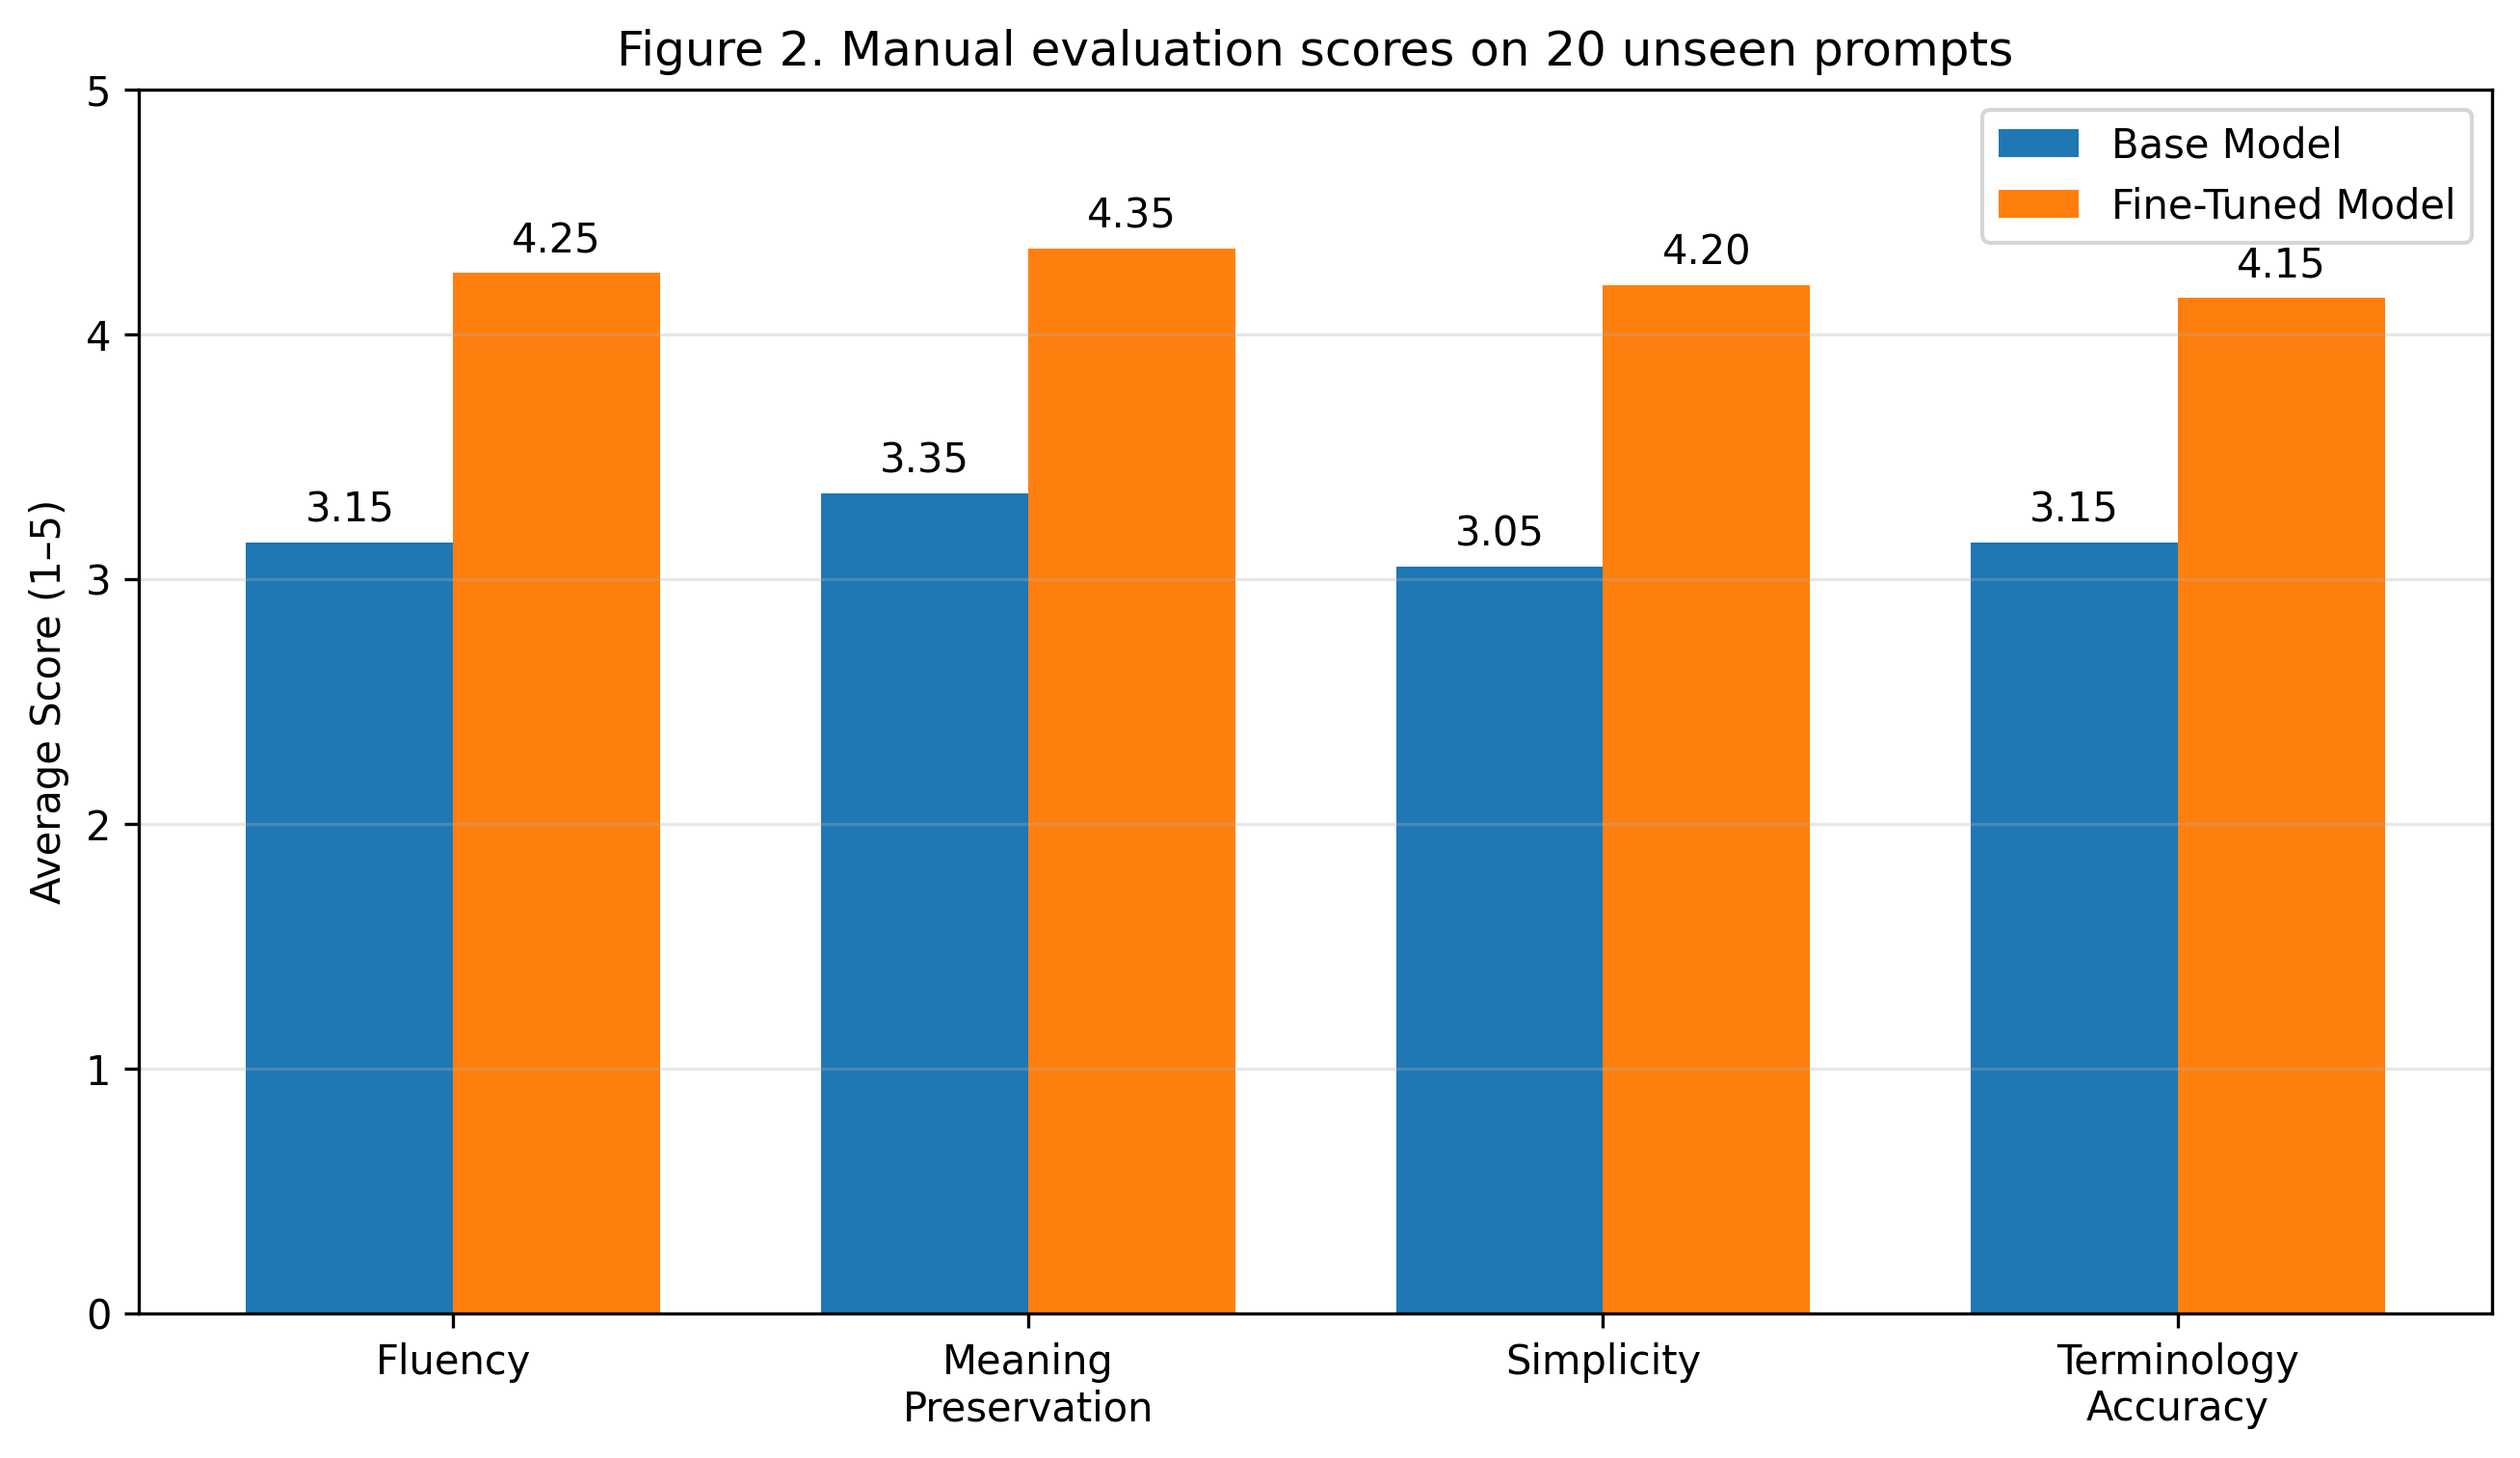
\includegraphics[width=\linewidth]{figure2_results_bar_chart.png}
\caption{Average manual evaluation scores for the base and fine-tuned models across the four evaluation dimensions.}
\label{fig:score_chart}
\end{figure}

\subsection{Qualitative Observations}

Qualitative inspection revealed three recurring patterns.

First, the fine-tuned model improved most clearly in structured domains with relatively stable terminology. In examples involving CDN-related web infrastructure, web servers, HTTP, cloud computing, and operating systems, the model more often generated correct Arabic technical terms while preserving the general meaning of the source. These domains appeared to benefit from glossary-guided prompting because the mapping between concept and preferred term was relatively explicit.

Second, the fine-tuned model often produced cleaner Arabic than the baseline. Earlier experiments had shown mixed-language contamination and unstable lexical substitutions. In the final system, these issues were reduced in several web-related, cloud, and infrastructure examples, although they did not disappear completely in all cases.

Third, improvements were less consistent in more abstract conceptual domains, particularly object-oriented programming. In some cases, the model still generated partially inaccurate conceptual paraphrases even when technical terms such as \textit{classe} and \textit{héritage} were correctly mapped. This suggests that terminology control alone is not sufficient for all concept types.

\subsection{Example Comparison}

A representative CDN example illustrates the gain clearly.

\textbf{Source text:}

\begin{quote}
Un CDN distribue le contenu web sur plusieurs serveurs afin d’améliorer la vitesse de chargement.
\end{quote}

\textbf{Base model output:}

\begin{quote}
\textarabic{ال \textenglish{CDN} ي \textenglish{Distribue} المحتوى الالكتروني على عدة خادم لتحسين سرعة التحميل.}
\end{quote}

\textbf{Fine-tuned output:}

\begin{quote}
\textarabic{شبكة توزيع المحتوى توزع المحتوى عبر عدة خوادم لتحسين سرعة تحميل المحتوى.}
\end{quote}

In this example, the fine-tuned output rendered the key domain term correctly, removed obvious multilingual contamination, and produced a clearer student-facing explanation.

A web-server example showed a similar pattern:

\textbf{Source text:}

\begin{quote}
Quand un utilisateur visite un site, le serveur web envoie la page au navigateur.
\end{quote}

\textbf{Fine-tuned output:}

\begin{quote}
\textarabic{خادم الويب يرسل صفحات الويب إلى المتصفحات عندما يزور المستخدم موقعًا.}
\end{quote}

Here again, the critical technical term was rendered correctly and the explanation was more fluent and comprehensible than the baseline.

\begin{table}[H]
\caption{Qualitative comparison examples across selected prompts.}
\label{tab:qual_examples}
\centering
\begin{tabular}{p{0.12\textwidth} p{0.24\textwidth} p{0.27\textwidth} p{0.27\textwidth}}
\toprule
\textbf{Topic} & \textbf{Source Text} & \textbf{Base Output} & \textbf{Fine-Tuned Output} \\
\midrule
CDN & Un CDN distribue le contenu web sur plusieurs serveurs afin d’améliorer la vitesse de chargement. & \textarabic{ال \textenglish{CDN} ي \textenglish{Distribue} المحتوى الالكتروني على عدة خادم لتحسين سرعة التحميل.} & \textarabic{شبكة توزيع المحتوى توزع المحتوى عبر عدة خوادم لتحسين سرعة تحميل المحتوى.} \\

Web Server & Quand un utilisateur visite un site, le serveur web envoie la page au navigateur. & \textarabic{عندما يزور المستخدم موقعًا، يرسل خادم الويب صفحةً ويبًا إلى متصفح المستخدم.} & \textarabic{خادم الويب يرسل صفحات الويب إلى المتصفحات عندما يزور المستخدم موقعًا.} \\

Cloud Computing & Le cloud permet de stocker et traiter les données sur des serveurs distants. & \textarabic{الحوسبة السحابية تسمح بتحقيق تخزين ومعالجة البيانات على خادم خارجي.} & \textarabic{الحوسبة السحابية تسمح بحفظ ومعالجة البيانات على خوادم آمنة في الإنترنت.} \\

Operating Systems & Le système d'exploitation gère les ressources matérielles et logicielles de l’ordinateur. & \textarabic{نظام التشغيل ي \textenglish{manage} الموارد المادية والمعنوية للجهاز.} & \textarabic{نظام التشغيل يتحكم في موارد النظام المادية والبرمجية.} \\

OOP (Limitation) & Une classe définit les propriétés et les méthodes qu’un objet peut posséder. & \textarabic{أحد الصنف يحدد الخصائص والدلالات التي يمكن أن تمتلكها الكائن.} & \textarabic{الصنف يحدد الخصائص والعمليات التي يمكن أن يمتلكها الكائن.} \\
\bottomrule
\end{tabular}
\end{table}

\section{Discussion}

The findings of this study indicate that glossary-guided fine-tuning can improve the simplification of IT educational content into Arabic for Moroccan learners. Across the 20 unseen evaluation prompts, the fine-tuned model outperformed the base Qwen2.5-1.5B-Instruct model on all four evaluation dimensions: fluency, meaning preservation, simplicity, and terminology accuracy. These gains suggest that the proposed approach did more than merely produce outputs that looked more Arabic. Rather, it improved several aspects of pedagogical quality that matter directly for technical explanation.

A central insight is that terminology guidance played an important role in the overall improvement. The baseline model was often able to produce partially understandable Arabic, but its outputs frequently showed lexical instability, code-mixing, and inconsistent rendering of technical terms. This problem was especially visible in web-related, infrastructure, and security prompts, where a mistranslated or unstable term could distort the underlying concept. By incorporating a domain glossary into prompt construction during dataset preparation, the fine-tuned model became more consistent in selecting appropriate Arabic technical terminology. The quantitative improvement in terminology accuracy, together with the qualitative comparison examples, supports this interpretation.

The gain in simplicity is equally significant. The goal of the system was not literal translation from French into Arabic, but pedagogical reformulation: preserving technical meaning while making explanations clearer and easier to understand. The fine-tuned model showed its strongest average improvement in simplicity, which suggests that it learned part of the intended educational rewriting behavior rather than only memorizing vocabulary mappings. This is particularly relevant in the Moroccan context, where many learners encounter IT concepts through French terminology even though their strongest language of conceptual access is often Arabic. In such settings, simplification quality depends not only on lexical substitution, but also on sentence structure, conceptual clarity, and the ability to avoid unnecessary linguistic complexity.

The qualitative results nevertheless show a mixed pattern rather than uniform success. In structured domains with relatively stable terminology, such as CDN-related web infrastructure, web servers, HTTP, cloud computing, and operating systems, the fine-tuned model generally produced clearer and more stable outputs than the baseline. In these cases, glossary guidance seems to have helped because the mapping between source concept and preferred Arabic term was relatively explicit. However, the improvement was not consistent in every terminology-heavy example. The SQL prompt, for instance, still showed code-mixing in the fine-tuned output, and the firewall example remained awkward despite being cleaner than the baseline in some respects. These cases indicate that terminology control helps, but does not by itself guarantee strong simplification.

A similar limitation appears in more abstract conceptual domains, especially object-oriented programming. In several cases, the fine-tuned model produced better technical wording than the baseline, but still struggled with conceptual precision. This suggests that abstract relational concepts are harder to simplify than terminology-heavy infrastructure examples. Correct term selection is useful, but it does not fully solve the problem of pedagogical explanation when the concept itself requires deeper restructuring or richer contextualization. In other words, the current approach appears most effective when the source concept can be anchored to relatively explicit domain vocabulary, and less reliable when conceptual understanding depends on more abstract semantic relations.

The study also highlights the practical value of using a small, locally adaptable model. The system was built on Qwen2.5-1.5B-Instruct and fine-tuned with LoRA in the MLX ecosystem on consumer Apple Silicon hardware. This matters because many educational settings, especially in low-resource or institutionally constrained environments, may not have access to large-scale compute infrastructure or proprietary API-based systems. The present results show that a compact model, when guided by curated task-specific data and terminology support, can still achieve meaningful improvements in educational text generation. This contributes to the broader argument that locally runnable and resource-aware Arabic educational NLP systems are both feasible and useful.

At the same time, the study has several limitations. First, the training dataset was intentionally small, containing only 150 paired examples. While this was sufficient for a proof-of-concept study, it limits coverage across subdomains, explanation styles, and difficulty levels. Second, the evaluation relied on manual scoring over 20 unseen prompts. This is acceptable for an initial prototype, but it does not provide the robustness of a larger benchmark or a multi-rater evaluation design. Third, the outputs were evaluated for linguistic and pedagogical quality, not for downstream learning outcomes. The study therefore shows improved simplification performance, but it does not yet establish whether learners who use such outputs would achieve better comprehension, retention, or academic performance.

Another limitation concerns linguistic scope. The target outputs were written in Modern Standard Arabic, whereas actual classroom support in Morocco may involve dynamic interaction among MSA, Darija, French, and sometimes English. The choice of MSA was appropriate for formal educational content and for maintaining linguistic consistency, but future systems may benefit from controlled adaptation across multiple varieties depending on learner profile, subject, or instructional context. In addition, the present work focused on glossary-guided prompting and LoRA fine-tuning only. It did not compare these choices against alternative strategies such as retrieval augmentation, instruction-only prompting, or synthetic data expansion.

Overall, the results support a cautious but clear conclusion: lightweight glossary-guided fine-tuning is a promising strategy for improving the accessibility of technical educational content in multilingual contexts such as Morocco. The contribution of this work lies not only in the numerical improvements reported, but also in showing that language accessibility in IT education can be treated as a concrete NLP design problem. By combining curated paired data, terminology control, and parameter-efficient adaptation, the study offers a practical starting point for future educational tools that support technical learning in a language learners understand more comfortably.

\section{Conclusion}

This paper presented a lightweight NLP approach for simplifying IT educational content into clear Modern Standard Arabic for Moroccan learners. Motivated by the linguistic gap between the language in which many students most easily construct technical understanding and the French- or English-dominant language of instruction, the study proposed a glossary-guided fine-tuning pipeline based on Qwen2.5-1.5B-Instruct and LoRA adaptation. A custom dataset of 150 paired examples was constructed across ten IT domains, and a domain glossary was integrated into prompt construction to improve the consistency of Arabic technical terminology.

The evaluation results showed that the fine-tuned model outperformed the base model on 20 unseen prompts across fluency, meaning preservation, simplicity, and terminology accuracy. The largest gain appeared in simplicity, suggesting that the model learned not only to render content in Arabic, but also to make explanations more pedagogically accessible. The qualitative examples further showed that glossary guidance often reduced multilingual drift and improved terminology stability in several important domains, particularly those with relatively explicit technical vocabulary, although these improvements were not uniform across all prompts.

The main contribution of the paper is therefore twofold. On the educational side, it shows that native-language support for technical learning can be approached through focused simplification rather than only through broad language-policy debates. On the computational side, it demonstrates that a small instruction-tuned language model can be adapted for a specialized Arabic educational task using limited data and modest hardware. This is especially relevant for contexts where scalable, low-cost, and locally runnable educational AI solutions are needed.

At the same time, the present work should be understood as a proof-of-concept study. The dataset remains limited in size, the evaluation is based on manual rubric scoring, and no classroom experiment was conducted to measure effects on learner understanding. Future work should therefore expand the corpus, improve coverage of abstract IT concepts, include multiple human raters, and investigate how such simplification systems perform in real educational settings. It would also be valuable to explore extensions toward bilingual or adaptive assistants that combine simplification, explanation, terminology support, and formative feedback.

In summary, the study provides evidence that glossary-guided fine-tuning is a viable and useful approach for Arabic IT text simplification in the Moroccan context. By treating multilingual educational difficulty as an applied NLP problem, it opens a practical path toward more accessible and linguistically inclusive technical learning support.

\authorcontributions{Conceptualization, K.E. and S.Z.; methodology, K.E.; software, K.E.; validation, K.E. and S.Z.; formal analysis, K.E.; investigation, K.E.; resources, K.E.; data curation, K.E.; writing---original draft preparation, K.E.; writing---review and editing, K.E. and S.Z.; visualization, K.E.; supervision, S.Z. All authors have read and agreed to the published version of the manuscript.}

\funding{This research received no external funding.}

\institutionalreview{Not applicable.}

\informedconsent{Not applicable.}

\dataavailability{The data presented in this study are available from the corresponding author upon reasonable request.}

\acknowledgments{}

\conflictsofinterest{The authors declare no conflicts of interest.}

\abbreviations{Abbreviations}{
\noindent
\begin{tabular}{@{}ll}
IT & Information Technology\\
MSA & Modern Standard Arabic\\
NLP & Natural Language Processing\\
LLM & Large Language Model\\
LoRA & Low-Rank Adaptation\\
CDN & Content Delivery Network
\end{tabular}
}

\reftitle{References}
\bibliography{references}

\PublishersNote{}

\end{document}